

\tikzset{every picture/.style={line width=0.75pt}} %set default line width to 0.75pt        

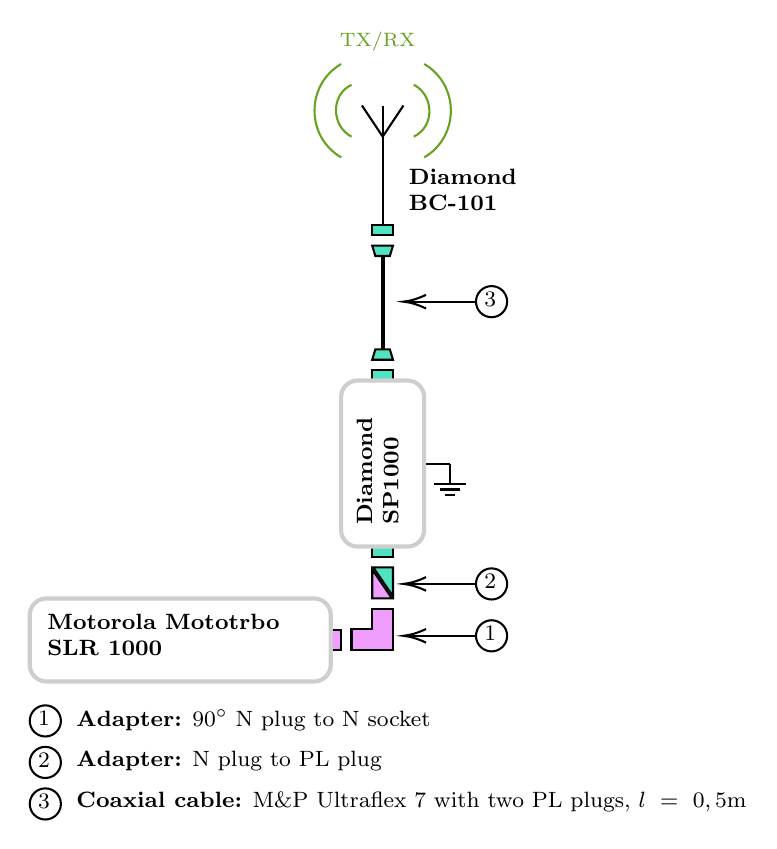
\begin{tikzpicture}[x=0.75pt,y=0.75pt,yscale=-1,xscale=1]
%uncomment if require: \path (0,463); %set diagram left start at 0, and has height of 463

%Straight Lines [id:da2117409366899652] 
\draw    (345,270) -- (357.5,270) ;
%Straight Lines [id:da19758281728068594] 
\draw    (357.5,270) -- (357.5,280) ;
%Straight Lines [id:da9706348152903634] 
\draw    (350,280) -- (365,280) ;
%Straight Lines [id:da9955066685628202] 
\draw    (352.5,282.5) -- (362.5,282.5) ;
%Straight Lines [id:da3542838525324348] 
\draw    (355,285) -- (360,285) ;

%Shape: Rectangle [id:dp5195215226134675] 
\draw  [fill={rgb, 255:red, 80; green, 227; blue, 194 }  ,fill opacity=1 ] (320,230) -- (320,225) -- (330,225) -- (330,230) -- cycle ;
%Shape: Rectangle [id:dp04379129192102571] 
\draw  [fill={rgb, 255:red, 80; green, 227; blue, 194 }  ,fill opacity=1 ] (320,315) -- (320,310) -- (330,310) -- (330,315) -- cycle ;
%Rounded Rect [id:dp609897861214854] 
\draw  [color={rgb, 255:red, 206; green, 206; blue, 206 }  ,draw opacity=1 ][line width=1.5]  (313,310) .. controls (308.58,310) and (305,306.42) .. (305,302) -- (305,238) .. controls (305,233.58) and (308.58,230) .. (313,230) -- (337,230) .. controls (341.42,230) and (345,233.58) .. (345,238) -- (345,302) .. controls (345,306.42) and (341.42,310) .. (337,310) -- cycle ;


%Straight Lines [id:da8216628264555428] 
\draw    (325.04,97.5) -- (325.04,157.5) ;
%Straight Lines [id:da11975977315738118] 
\draw    (315.04,97.5) -- (325.04,112.5) ;
%Straight Lines [id:da2623857929633875] 
\draw    (325.04,112.5) -- (335.04,97.5) ;
%Curve Lines [id:da9838947299311864] 
\draw [color={rgb, 255:red, 101; green, 162; blue, 30 }  ,draw opacity=1 ]   (340.04,87.5) .. controls (349.76,92.5) and (350.33,107.64) .. (340.04,112.5) ;
%Curve Lines [id:da48333252009100747] 
\draw [color={rgb, 255:red, 101; green, 162; blue, 30 }  ,draw opacity=1 ]   (345.04,77.5) .. controls (362.29,87.63) and (362.04,112.63) .. (345.04,122.5) ;

%Curve Lines [id:da06276736990916465] 
\draw [color={rgb, 255:red, 101; green, 162; blue, 30 }  ,draw opacity=1 ]   (310.04,112.5) .. controls (300.33,107.5) and (299.76,92.36) .. (310.04,87.5) ;
%Curve Lines [id:da8544747440552438] 
\draw [color={rgb, 255:red, 101; green, 162; blue, 30 }  ,draw opacity=1 ]   (305.04,122.5) .. controls (287.79,112.38) and (288.04,87.37) .. (305.04,77.5) ;

%Shape: Rectangle [id:dp5540086456806208] 
\draw  [fill={rgb, 255:red, 80; green, 227; blue, 194 }  ,fill opacity=1 ] (320.04,155) -- (330.04,155) -- (330.04,160) -- (320.04,160) -- cycle ;
%Shape: Rectangle [id:dp17515633991893775] 
\draw  [fill={rgb, 255:red, 239; green, 158; blue, 255 }  ,fill opacity=1 ] (300,350) -- (305,350) -- (305,360) -- (300,360) -- cycle ;
%Rounded Rect [id:dp7223835974557309] 
\draw  [color={rgb, 255:red, 206; green, 206; blue, 206 }  ,draw opacity=1 ][line width=1.5]  (155,343) .. controls (155,338.58) and (158.58,335) .. (163,335) -- (292,335) .. controls (296.42,335) and (300,338.58) .. (300,343) -- (300,367) .. controls (300,371.42) and (296.42,375) .. (292,375) -- (163,375) .. controls (158.58,375) and (155,371.42) .. (155,367) -- cycle ;


%Shape: Path Data [id:dp2172730430252452] 
\draw  [fill={rgb, 255:red, 239; green, 158; blue, 255 }  ,fill opacity=1 ] (310,360) -- (310,349.67) -- (320,349.67) -- (320,340) -- (330,340) -- (330,360) -- (310,360) -- cycle ;
%Shape: Right Triangle [id:dp30746565461403486] 
\draw  [fill={rgb, 255:red, 80; green, 227; blue, 194 }  ,fill opacity=1 ] (320.48,320) -- (330,333.98) -- (330,320) -- cycle ;
%Shape: Right Triangle [id:dp7515173690048442] 
\draw  [fill={rgb, 255:red, 239; green, 158; blue, 255 }  ,fill opacity=1 ] (329.52,335) -- (320,321.02) -- (320,335) -- cycle ;

%Straight Lines [id:da9120395561613033] 
\draw [line width=1.5]    (325,170) -- (325,215) ;
%Shape: Trapezoid [id:dp9006012786033941] 
\draw  [fill={rgb, 255:red, 80; green, 227; blue, 194 }  ,fill opacity=1 ][line width=0.75]  (330,165) -- (328.5,170) -- (321.5,170) -- (320,165) -- cycle ;
%Shape: Trapezoid [id:dp20960810518276118] 
\draw  [fill={rgb, 255:red, 80; green, 227; blue, 194 }  ,fill opacity=1 ][line width=0.75]  (320,220) -- (321.5,215) -- (328.5,215) -- (330,220) -- cycle ;

%Straight Lines [id:da35692414312633214] 
\draw    (370,353) -- (337,353) ;
\draw [shift={(335,353)}, rotate = 360] [color={rgb, 255:red, 0; green, 0; blue, 0 }  ][line width=0.75]    (10.93,-3.29) .. controls (6.95,-1.4) and (3.31,-0.3) .. (0,0) .. controls (3.31,0.3) and (6.95,1.4) .. (10.93,3.29)   ;
%Shape: Circle [id:dp44275798239943964] 
\draw   (370,353) .. controls (370,348.86) and (373.36,345.5) .. (377.5,345.5) .. controls (381.64,345.5) and (385,348.86) .. (385,353) .. controls (385,357.14) and (381.64,360.5) .. (377.5,360.5) .. controls (373.36,360.5) and (370,357.14) .. (370,353) -- cycle ;


%Shape: Circle [id:dp08416294362563437] 
\draw   (370,328) .. controls (370,323.86) and (373.36,320.5) .. (377.5,320.5) .. controls (381.64,320.5) and (385,323.86) .. (385,328) .. controls (385,332.14) and (381.64,335.5) .. (377.5,335.5) .. controls (373.36,335.5) and (370,332.14) .. (370,328) -- cycle ;

%Straight Lines [id:da011949664490807699] 
\draw    (370,328) -- (337,328) ;
\draw [shift={(335,328)}, rotate = 360] [color={rgb, 255:red, 0; green, 0; blue, 0 }  ][line width=0.75]    (10.93,-3.29) .. controls (6.95,-1.4) and (3.31,-0.3) .. (0,0) .. controls (3.31,0.3) and (6.95,1.4) .. (10.93,3.29)   ;

%Shape: Circle [id:dp29561759695484313] 
\draw   (370,192) .. controls (370,187.86) and (373.36,184.5) .. (377.5,184.5) .. controls (381.64,184.5) and (385,187.86) .. (385,192) .. controls (385,196.14) and (381.64,199.5) .. (377.5,199.5) .. controls (373.36,199.5) and (370,196.14) .. (370,192) -- cycle ;

%Straight Lines [id:da6708191132816714] 
\draw    (370,192) -- (337,192) ;
\draw [shift={(335,192)}, rotate = 360] [color={rgb, 255:red, 0; green, 0; blue, 0 }  ][line width=0.75]    (10.93,-3.29) .. controls (6.95,-1.4) and (3.31,-0.3) .. (0,0) .. controls (3.31,0.3) and (6.95,1.4) .. (10.93,3.29)   ;

%Shape: Circle [id:dp6925244802161248] 
\draw   (155,394) .. controls (155,389.86) and (158.36,386.5) .. (162.5,386.5) .. controls (166.64,386.5) and (170,389.86) .. (170,394) .. controls (170,398.14) and (166.64,401.5) .. (162.5,401.5) .. controls (158.36,401.5) and (155,398.14) .. (155,394) -- cycle ;

%Shape: Circle [id:dp5144865887931986] 
\draw   (155,414) .. controls (155,409.86) and (158.36,406.5) .. (162.5,406.5) .. controls (166.64,406.5) and (170,409.86) .. (170,414) .. controls (170,418.14) and (166.64,421.5) .. (162.5,421.5) .. controls (158.36,421.5) and (155,418.14) .. (155,414) -- cycle ;

%Shape: Circle [id:dp2881120818061964] 
\draw   (155,434) .. controls (155,429.86) and (158.36,426.5) .. (162.5,426.5) .. controls (166.64,426.5) and (170,429.86) .. (170,434) .. controls (170,438.14) and (166.64,441.5) .. (162.5,441.5) .. controls (158.36,441.5) and (155,438.14) .. (155,434) -- cycle ;



% Text Node
\draw (157.5,428) node [anchor=north west][inner sep=0.75pt]  [font=\footnotesize] [align=left] {3};
% Text Node
\draw (157.5,408) node [anchor=north west][inner sep=0.75pt]  [font=\footnotesize] [align=left] {2};
% Text Node
\draw (157.5,388) node [anchor=north west][inner sep=0.75pt]  [font=\footnotesize] [align=left] {1};
% Text Node
\draw (372.5,186) node [anchor=north west][inner sep=0.75pt]  [font=\footnotesize] [align=left] {3};
% Text Node
\draw (372.5,322) node [anchor=north west][inner sep=0.75pt]  [font=\footnotesize] [align=left] {2};
% Text Node
\draw (372.5,347) node [anchor=north west][inner sep=0.75pt]  [font=\footnotesize] [align=left] {1};
% Text Node
\draw (302.89,60.5) node [anchor=north west][inner sep=0.75pt]  [font=\scriptsize,color={rgb, 255:red, 101; green, 162; blue, 30 }  ,opacity=1 ] [align=left] {TX/RX};
% Text Node
\draw (311,301) node [anchor=north west][inner sep=0.75pt]  [font=\footnotesize,rotate=-270] [align=left] {\textbf{Diamond}\\\textbf{SP1000}};
% Text Node
\draw (162,341) node [anchor=north west][inner sep=0.75pt]  [font=\footnotesize] [align=left] {\textbf{Motorola Mototrbo}\\\textbf{SLR 1000}};
% Text Node
\draw (336.2,126.5) node [anchor=north west][inner sep=0.75pt]  [font=\footnotesize] [align=left] {\textbf{Diamond }\\\textbf{BC-101}};
% Text Node
\draw (176,427) node [anchor=north west][inner sep=0.75pt]  [font=\footnotesize] [align=left] {\textbf{Coaxial cable:} M\&P Ultraflex 7 with two PL plugs, $\displaystyle l\ =\ 0,5\mathrm{m}$};
% Text Node
\draw (176,407) node [anchor=north west][inner sep=0.75pt]  [font=\footnotesize] [align=left] {\textbf{Adapter:} N plug to PL plug};
% Text Node
\draw (176,387) node [anchor=north west][inner sep=0.75pt]  [font=\footnotesize] [align=left] {\textbf{Adapter:} $\displaystyle 90^{\circ }$ N plug to N socket};


\end{tikzpicture}
